\section{Statistical Analysis of Experiment \#2}\label{sec:Stat2}
In this section the analysis of the results from experiment 2 will be conducted. The overall expectation is that the results will be relatively similar to the findings from \cref{sec:Stat1}. Some divinations are within our expectations as experiment 2 not oly disables the C-State, but is also only done on the workstation.Firstly the normal distribution for experiment 2 will be analyzed using the Shapiro-Wilk test.

\subsection{Normal distribution}\label{subsec:NormalDist2}
In this section the analysis of the results from experiment 2 will be conducted. Firstly the normal distribution for experiment 2 will be analyzed using the Shapiro-Wilk test. 

\paragraph{Expectations}
The expectations is that the distribution will not be normally distributed, this is because experiment 1 in \cref{sec:Stat1} was not always normally distributed, we would not expected this experiment to differ much in that aspects. 

\paragraph{Results}
The results from the Sharpiro Wilk can be seen herr \cref{tab:NormalDist2}
\begin{table}[]
    \begin{tabular}{||c|c|c|c|c|c||}    \hline
    &\textbf{TestCaseIdle}&\textbf{BinaryTrees}&\textbf{FannkuchRedux}&\textbf{Nbody}&\textbf{Fasta}\\ [0.5ex] \hline
    \hline \textbf{IntelPowerGadget}&0.0&0.9103&0.1293&0.0002&0.8291\\
    \textbf{HardwareMonitor}&0.0213&0.1345&0.0492&0.3209&0.0\\
    \textbf{Clamp Win}&0.0034&0.0023&0.012&0.8143&0.5335\\
    \textbf{RAPL}&0.1899&0.5744&0.0015&0.9437&0.0518\\
    \textbf{Clamp Lin}&0.4601&0.0004&0.0&0.1006&0.0002\\ \hline \end{tabular}
    \caption{P values for the normal distribution for the Workstation in Ex2}
    \label{tab:NormDist2}
\end{table} 
As can be seen in \cref{tab:NormDist2}, the data is not normally distributed the data from experiment 2 is generally further away from being normally distributed than in experiment 1. This is not that surprising given that experiment 2 contain fewer samples as these were not needed as found in \cref{subsec:CockUse}.

\subsection{Independence Test}\label{subsec:independence2}
It was found in \cref{subsec:NormalDist2}, that the data for experiment 2 was not normally distributed, because of this the Mann Whitney U Test will be used to test independence just like in \cref{subsec:independence1}.

\paragraph{Expectations}
For the MannWhitney U test we would expect very similar results to the results from experiment 1, where the null hypotheses can be rejected in most of the cases. This is because the changes between in experiment 1 and experiment 2 would not change the independence of the data, so should not change the result remarkably

\paragraph{Results}
The results from the MannWhitney U test can be seen here in \cref{tab:HeatFannkuchRedux2}, the results from the rest of the test cases can eb found in the appendix.
\begin{figure}
    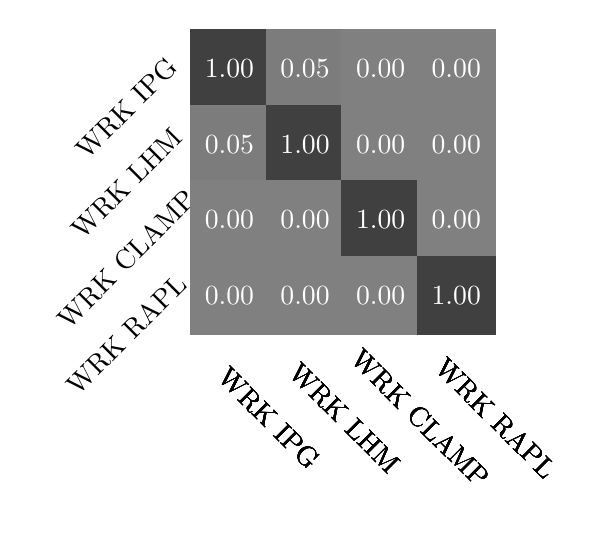
\begin{tikzpicture}[scale=0.6]
      \foreach \y [count=\n] in {{1.00, 0.05, 0.00, 0.00},{0.05, 1.00, 0.00, 0.00},{0.00, 0.00, 1.00, 0.00},{0.00, 0.00, 0.00, 1.00},} {
      % column labels
      \foreach \a [count=\n] in {WRK IPG,WRK LHM,WRK CLAMP,WRK RAPL} {
        \node[minimum size=10mm, xshift=0.5cm, rotate=-45] at (\n*1.6, -9.0) {\a};
      }
      % heatmap tiles
      \foreach \x [count=\m] in \y {
        \pgfmathsetmacro{\xa }{(\x + 1) / 2 * 100}
        \node[fill=darkgray!\xa!lightgray, minimum size=10mm, text=white, font={\normalsize}] at (\m*1.6,-\n*1.6) {\x};
      }
    }
      % row labels
      \foreach \a [count=\i] in {WRK IPG,WRK LHM,WRK CLAMP,WRK RAPL} {
        \node[minimum size=10mm, xshift=-0.35cm, yshift=-0.5cm, rotate=45] at (0,-\i*1.6) {\a};
      }
    \end{tikzpicture}
    \label{tab:HeatFannkuchRedux2}
\end{figure}
The shown table in \cref{tab:HeatFannkuchRedux2}, is again from the FannkuchRedux Test Case as in \cref{sec:Stat1}. Again we see a similar tendency in that for most cases we can reject $H_0$, but for experiment 2 there are a few more cases where we cannot reject $H_0$. Once possible reason why that might be the case is that there are fewer samples in experiment 2 so outlier have a larger effect on the Ex1Statistics.

\subsection{Correlation}\label{subsec:correlation2}
In this section the correlation between teh different measurement instrument will be conducted for experiment 2. The Kendall Tau correlation coefficients will again be used as it was in \cref{subsec:correlation1}

\paragraph{Expectations}
The expectations for the correlations in Experiment 2 is that they are either are a bit more correlated since the uncertainty's of the C-Stats have been removed, or that it will remain nearly exactly the same.
\paragraph{Results}
The calculated Correlations for experiments 2 can be seen in \cref{tab:correlationWork2}.
\begin{figure}
    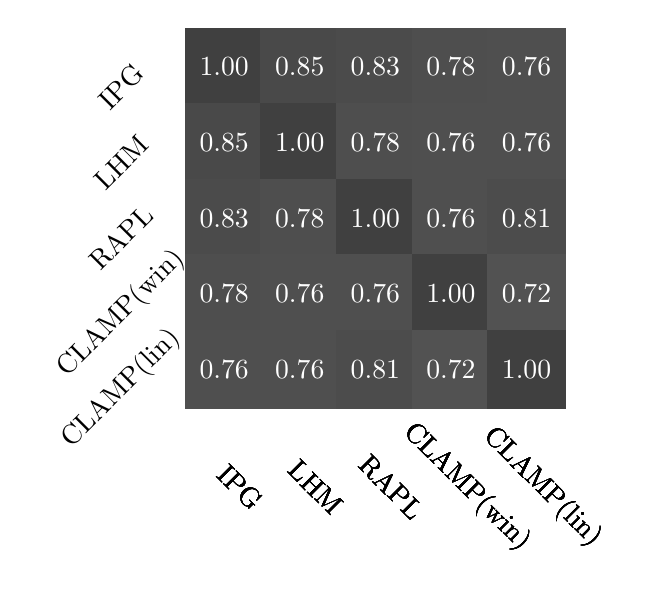
\begin{tikzpicture}[scale=0.6]
      \foreach \y [count=\n] in {{1.00, 0.85, 0.83, 0.78, 0.76},{0.85, 1.00, 0.78, 0.76, 0.76},{0.83, 0.78, 1.00, 0.76, 0.81},{0.78, 0.76, 0.76, 1.00, 0.72},{0.76, 0.76, 0.81, 0.72, 1.00},} {
      % column labels
      \foreach \a [count=\n] in {IPG,LHM,RAPL,CLAMP(win),CLAMP(lin)} {
        \node[minimum size=10mm, xshift=0.2cm, rotate=-45] at (\n*1.6, -10.5) {\a};
      }
      % heatmap tiles
      \foreach \x [count=\m] in \y {
        \pgfmathsetmacro{\xa }{(\x + 1) / 2 * 100}
        \node[fill=darkgray!\xa!lightgray, minimum size=10mm, text=white, font={\normalsize}] at (\m*1.6,-\n*1.6) {\x};
      }
    }
      % row labels
      \foreach \a [count=\i] in {IPG,LHM,RAPL,CLAMP(win),CLAMP(lin)} {
        \node[minimum size=10mm, xshift=-0.35cm, yshift=-0.25cm, rotate=45] at (0,-\i*1.6) {\a};
      }
    \end{tikzpicture}
    \label{tab:correlationWork2}
\end{figure}
These results generally look very similar to the number obtained from experiment 1 in \cref{subsec:correlation1}. 
The average correlation from experiments on the workstation are:
$$AvgCoefEx1 = (0.81+0.80+0.77+0.71+0.80+0.78+0.71+0.77+0.72+0.70)/10 = 0.757$$
$$AvgCoefEx2 = (0.85+0.83+0.78+0.76+0.78+0.76+0.76+0.76+0.81+0.72)/10 = 0.781$$
These seem to generally show the a higher correlations between the different DUTs and their measurement instruments, but a more in-depth analysis will be made in \cref{subsec:ResultStat2}

\subsection{Results}\label{subsec:ResultStat2}  
In this section teh results from \cref{subsec:correlation2}, will be analyzed and utilized to answer our research questions. 
\paragraph{RQ2}
When comparing the measurement instruments to each other the average correlation foreach instrument can be found. These will then be compared with the results from \cref{subsec:ResultStat1}, to see what effect disabling the C-States have had on the instruments.
\begin{itemize}
    \item \textbf{Experiment 1}
    \begin{itemize}
        \item $IPG = 0.772$ %0.81+0.80+0.77+0.71
        \item $LHM = 0.775$ %0.81+0.80+0.78+0.71
        \item $RAPL = 0.725$ %0.80+0.80+0.77+0.72
        \item $CLAMP(win) = 0.755$ %0.77+0.78+0.77+0.70
        \item $CLAMP(lin) = 0.710$ %0.71+0.71+0.72+0.70
    \end{itemize}
    \item \textbf{Experiment 2}
    \begin{itemize}
        \item $IPG = 0.805$ %0.85+0.83+0.78+0.76
        \item $LHM = 0.787$ %0.85+0.78+0.76+0.76
        \item $RAPL = 0.795$%0.83+0.78+0.76+0.81
        \item $CLAMP(win) = 0.755$ %0.78+0.76+0.76+0.72
        \item $CLAMP(lin) = 762$ % 0.76+0.76+0.81+0.72
    \end{itemize}
\end{itemize}
When looking at the average correlation foreach of the measurement instruments across the two experiments, experiment 2 have generally larger coefficients than experiment 1. Looking at these number using the Guildford scale, none of them change evaluation, but are alls still highly correlated to each other, as we expected.

\paragraph{RQ3}
When comparing the results based on the OS, we can observer some larger differences when compared with experiment 1. The OS that benefits the most in terms of correlation coefficients, when disabling the C-Stats is linux as both average correlation between RAPL and the rest of of the measurement instrument rises. This is mostly dues to an increase in the correlation RAPL have with the CLAMP(lin) which goes from $0.72$ to $0.81$. RAPL even gets a marginally smaller coefficients in some case, but the growth of it's correlation CLAMP(lin) out weight them.  Overall it seems that RAPL is the one most closely correlated with the hardware measurements while IPG is the one for Windows.





% \begin{table}[]
    \begin{tabular}{||c|c|c|c|c|c||}    \hline
    &\textbf{TestCaseIdle}&\textbf{BinaryTrees}&\textbf{FannkuchRedux}&\textbf{Nbody}&\textbf{Fasta}\\ [0.5ex] \hline
    \hline \textbf{IntelPowerGadget}&0.0&0.9103&0.1293&0.0002&0.8291\\
    \textbf{HardwareMonitor}&0.0213&0.1345&0.0492&0.3209&0.0\\
    \textbf{Clamp Win}&0.0034&0.0023&0.012&0.8143&0.5335\\
    \textbf{RAPL}&0.1899&0.5744&0.0015&0.9437&0.0518\\
    \textbf{Clamp Lin}&0.4601&0.0004&0.0&0.1006&0.0002\\ \hline \end{tabular}
    \caption{P values for the normal distribution for the Workstation in Ex2}
    \label{tab:NormDist2}
\end{table} 

% As can be seen in \cref{tab:NormDist2}, the data is not normally distributed the data from experiment 2 is generally further away from being normally distributed than the experiment 1. This is not that surprising given that experiment 2 contain less actual runs as these were not needed as found in \cref{subsec:CockUse}. 

% For the MannWhitney U test we would again expect very similar results to the results from experiment one, where the null hypotheses can be rejected in most of the cases.
% The results from the MannWhitney U test can be seen here in \cref{tab:HeatFannkuchRedux2}.
% \begin{figure}
    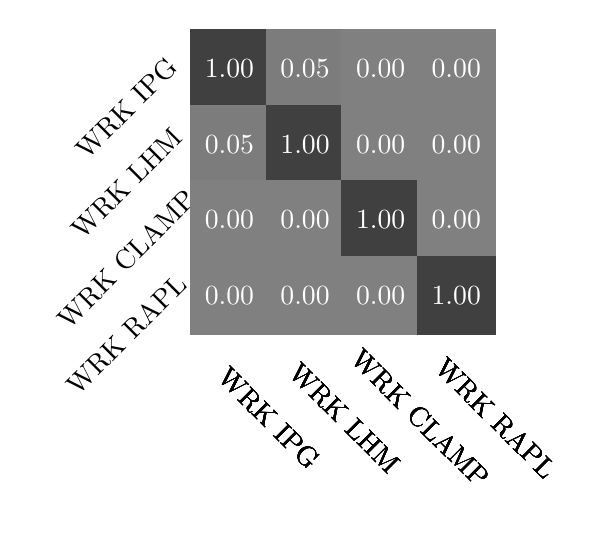
\begin{tikzpicture}[scale=0.6]
      \foreach \y [count=\n] in {{1.00, 0.05, 0.00, 0.00},{0.05, 1.00, 0.00, 0.00},{0.00, 0.00, 1.00, 0.00},{0.00, 0.00, 0.00, 1.00},} {
      % column labels
      \foreach \a [count=\n] in {WRK IPG,WRK LHM,WRK CLAMP,WRK RAPL} {
        \node[minimum size=10mm, xshift=0.5cm, rotate=-45] at (\n*1.6, -9.0) {\a};
      }
      % heatmap tiles
      \foreach \x [count=\m] in \y {
        \pgfmathsetmacro{\xa }{(\x + 1) / 2 * 100}
        \node[fill=darkgray!\xa!lightgray, minimum size=10mm, text=white, font={\normalsize}] at (\m*1.6,-\n*1.6) {\x};
      }
    }
      % row labels
      \foreach \a [count=\i] in {WRK IPG,WRK LHM,WRK CLAMP,WRK RAPL} {
        \node[minimum size=10mm, xshift=-0.35cm, yshift=-0.5cm, rotate=45] at (0,-\i*1.6) {\a};
      }
    \end{tikzpicture}
    \label{tab:HeatFannkuchRedux2}
\end{figure}
% The shown table in \cref{tab:HeatFannkuchRedux2}, is again from the FannkuchRedux Test Case as in \cref{subsec:Stat1}. Again we see a similar tendency in that for most cases we can reject $H_0$, but for experiment 2 there are a few more cases where we cannot reject $H_0$. Once possible reason why that might be the case is that there are fewer samples in experiment 2 so outlier have a larger effect on the Ex1Statistics.

% Finally for the Correlations between the measuring instruments, the expectations for the correlations in Experiment 2 is that they are either are a bit more correlated since the uncertainty's of the C-Stats have been removed, or that i will remain nearly exactly the same. The calculated Correlations for experiments 2 can be seen in \cref{tab:correlationWork2}.
% \begin{figure}
    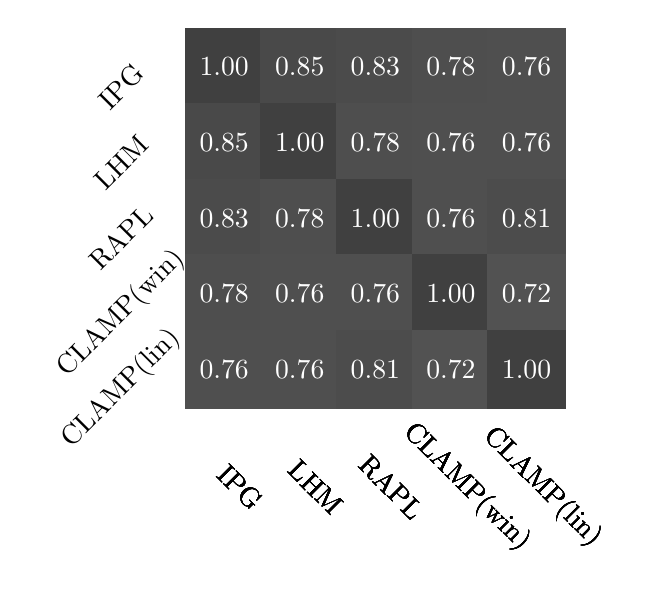
\begin{tikzpicture}[scale=0.6]
      \foreach \y [count=\n] in {{1.00, 0.85, 0.83, 0.78, 0.76},{0.85, 1.00, 0.78, 0.76, 0.76},{0.83, 0.78, 1.00, 0.76, 0.81},{0.78, 0.76, 0.76, 1.00, 0.72},{0.76, 0.76, 0.81, 0.72, 1.00},} {
      % column labels
      \foreach \a [count=\n] in {IPG,LHM,RAPL,CLAMP(win),CLAMP(lin)} {
        \node[minimum size=10mm, xshift=0.2cm, rotate=-45] at (\n*1.6, -10.5) {\a};
      }
      % heatmap tiles
      \foreach \x [count=\m] in \y {
        \pgfmathsetmacro{\xa }{(\x + 1) / 2 * 100}
        \node[fill=darkgray!\xa!lightgray, minimum size=10mm, text=white, font={\normalsize}] at (\m*1.6,-\n*1.6) {\x};
      }
    }
      % row labels
      \foreach \a [count=\i] in {IPG,LHM,RAPL,CLAMP(win),CLAMP(lin)} {
        \node[minimum size=10mm, xshift=-0.35cm, yshift=-0.25cm, rotate=45] at (0,-\i*1.6) {\a};
      }
    \end{tikzpicture}
    \label{tab:correlationWork2}
\end{figure}
% At an first these results look very similar to the once from experiment 1, but to verify these number more in depth we can compare the averages of the correlations as before.


% This slight increase in overall correlation matches up with our expectations as the added consistency in the experiments should help reduce inconsistencies. Generally the correlations are higher in experiment 2, but the correlation does fall in certain cases, these cases will be looked at a bit here.

% The first case is the $RAPL|CLAMP(win)$ which used to in experiment one to have a coefficients of $0.77$, but in Experiment 2 as $0.76$, while this is only a marginal decrease it could be caused by the fact that one measures linux and the other windows. Another one is $LHM|RAPL$ which went from $0.80$ to $0.78$ these measurements are again done on separate OSs. 

% So the divide between linux and windows seems to have gotten larger.   









